% Options for packages loaded elsewhere
\PassOptionsToPackage{unicode}{hyperref}
\PassOptionsToPackage{hyphens}{url}
%
\documentclass[
]{book}
\usepackage{amsmath,amssymb}
\usepackage{lmodern}
\usepackage{iftex}
\ifPDFTeX
  \usepackage[T1]{fontenc}
  \usepackage[utf8]{inputenc}
  \usepackage{textcomp} % provide euro and other symbols
\else % if luatex or xetex
  \usepackage{unicode-math}
  \defaultfontfeatures{Scale=MatchLowercase}
  \defaultfontfeatures[\rmfamily]{Ligatures=TeX,Scale=1}
\fi
% Use upquote if available, for straight quotes in verbatim environments
\IfFileExists{upquote.sty}{\usepackage{upquote}}{}
\IfFileExists{microtype.sty}{% use microtype if available
  \usepackage[]{microtype}
  \UseMicrotypeSet[protrusion]{basicmath} % disable protrusion for tt fonts
}{}
\makeatletter
\@ifundefined{KOMAClassName}{% if non-KOMA class
  \IfFileExists{parskip.sty}{%
    \usepackage{parskip}
  }{% else
    \setlength{\parindent}{0pt}
    \setlength{\parskip}{6pt plus 2pt minus 1pt}}
}{% if KOMA class
  \KOMAoptions{parskip=half}}
\makeatother
\usepackage{xcolor}
\IfFileExists{xurl.sty}{\usepackage{xurl}}{} % add URL line breaks if available
\IfFileExists{bookmark.sty}{\usepackage{bookmark}}{\usepackage{hyperref}}
\hypersetup{
  pdftitle={Data Privacy Handbook},
  pdfauthor={Utrecht University},
  hidelinks,
  pdfcreator={LaTeX via pandoc}}
\urlstyle{same} % disable monospaced font for URLs
\usepackage{longtable,booktabs,array}
\usepackage{calc} % for calculating minipage widths
% Correct order of tables after \paragraph or \subparagraph
\usepackage{etoolbox}
\makeatletter
\patchcmd\longtable{\par}{\if@noskipsec\mbox{}\fi\par}{}{}
\makeatother
% Allow footnotes in longtable head/foot
\IfFileExists{footnotehyper.sty}{\usepackage{footnotehyper}}{\usepackage{footnote}}
\makesavenoteenv{longtable}
\usepackage{graphicx}
\makeatletter
\def\maxwidth{\ifdim\Gin@nat@width>\linewidth\linewidth\else\Gin@nat@width\fi}
\def\maxheight{\ifdim\Gin@nat@height>\textheight\textheight\else\Gin@nat@height\fi}
\makeatother
% Scale images if necessary, so that they will not overflow the page
% margins by default, and it is still possible to overwrite the defaults
% using explicit options in \includegraphics[width, height, ...]{}
\setkeys{Gin}{width=\maxwidth,height=\maxheight,keepaspectratio}
% Set default figure placement to htbp
\makeatletter
\def\fps@figure{htbp}
\makeatother
\setlength{\emergencystretch}{3em} % prevent overfull lines
\providecommand{\tightlist}{%
  \setlength{\itemsep}{0pt}\setlength{\parskip}{0pt}}
\setcounter{secnumdepth}{5}
\usepackage{booktabs}
\ifLuaTeX
  \usepackage{selnolig}  % disable illegal ligatures
\fi
\usepackage[]{natbib}
\bibliographystyle{apalike}

\title{Data Privacy Handbook}
\author{Utrecht University}
\date{2021-11-05}

\begin{document}
\maketitle

{
\setcounter{tocdepth}{1}
\tableofcontents
}
\hypertarget{welcome}{%
\chapter*{Welcome!}\label{welcome}}
\addcontentsline{toc}{chapter}{Welcome!}

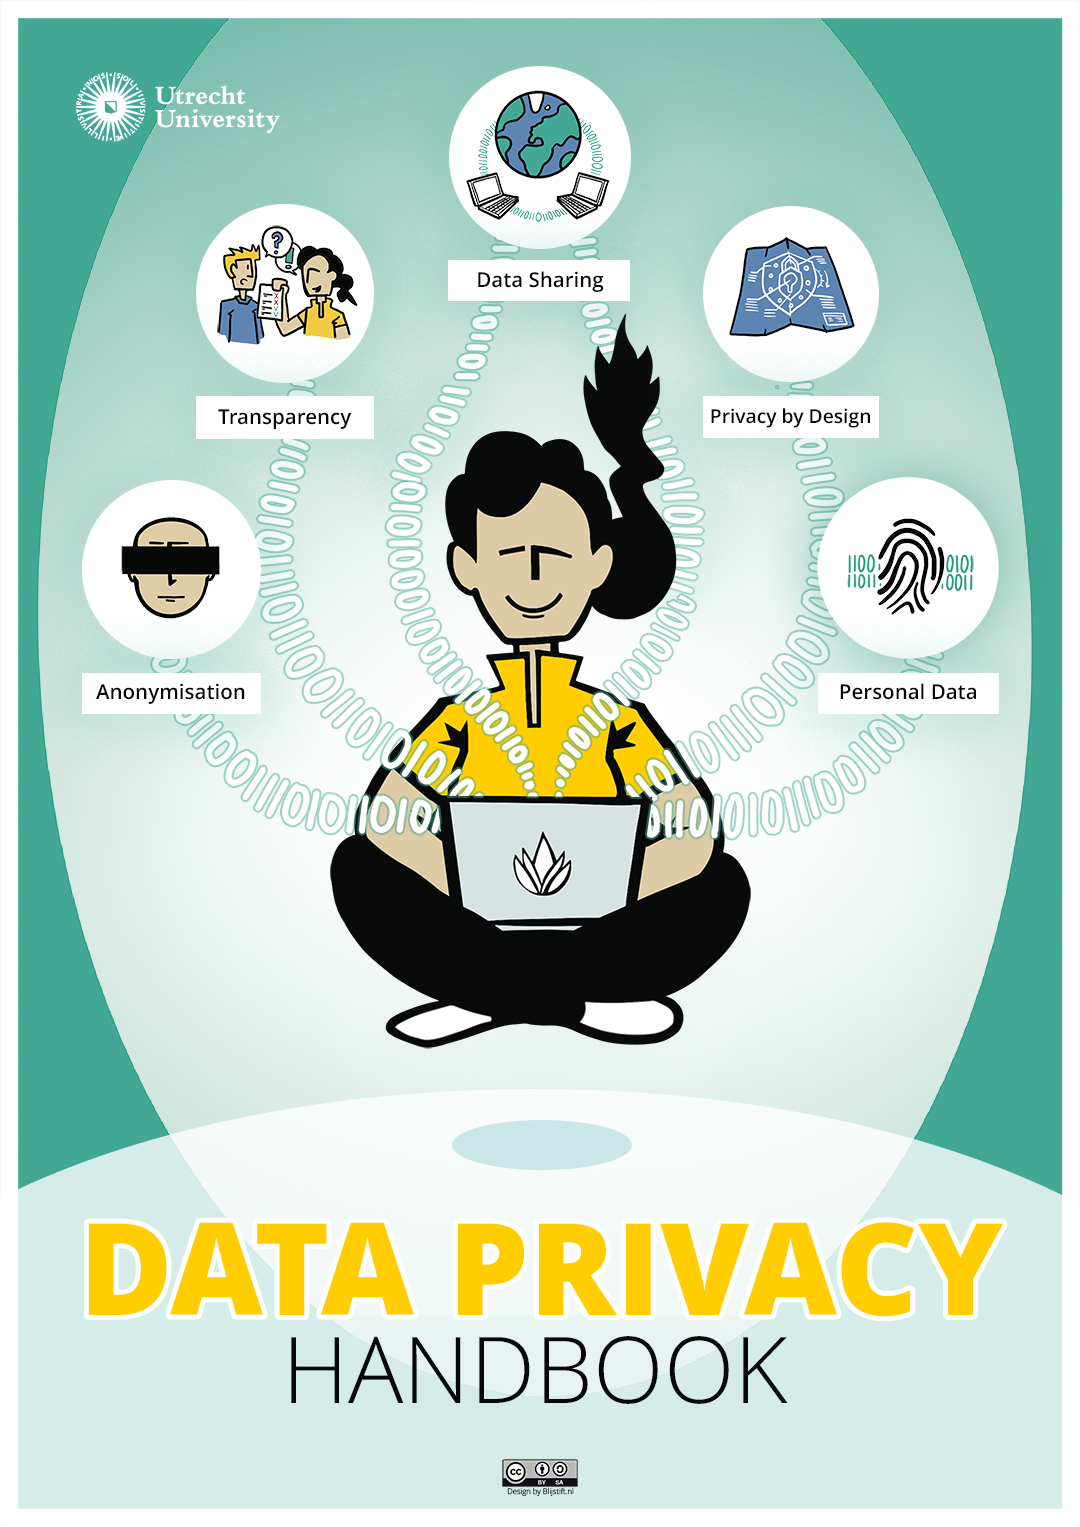
\includegraphics{img/cover-image-dph.png}

The Data Privacy Handbook is a guide on handling personal data in scientific
research, in line with European data protection and privacy regulations. It
consists of:

\begin{itemize}
\tightlist
\item
  A \textbf{knowledge base} which explains how the EU General Data Protection Regulation (GDPR, Dutch: Algemene Verordening Gegevensbescherming) applies to scientific research, including guidelines and good practices in carrying out GDPR-compliant scientific research;
\item
  An overview of privacy-enhancing \textbf{techniques \& tools} and practical guidance on their implementation;
\item
  \textbf{Use Cases} in the form of research projects with privacy-related issues, for which a reusable solution (e.g., tool, workflow) has been developed.
\end{itemize}

The Data Privacy Handbook synthesizes information across various sources and
presents it a \emph{practical} and \emph{actionable} format. This includes workflows,
tools, and practical translations of the GDPR , which could be used by researchers
and (data) support staff within Utrecht University and beyond.

This is an Utrecht University (UU) community-driven, open-source project.
You can visit our GitHub repository here.
We welcome feedback and contributions of any type, please read our
contributing guidelines
for more information.

The Data Privacy Handbook is an initiative of
Research Data Management Support
at the Utrecht University Library,
in collaboration with privacy and data experts at Utrecht University. It is part of a larger Data Privacy Project,
that aims to develop knowledge, tools, and experience on how researchers can and
should deal with personal data. This project is funded by the Utrecht University
Research IT Program and an NWO Digital Competence Center grant. You can read more
about the Data Privacy Project here.

\hypertarget{how-to-use-this-handbook}{%
\section{How to use this Handbook}\label{how-to-use-this-handbook}}

The Data Privacy Handbook aims to make knowledge and solutions on handling personal
data \emph{Findable, Accessible, Interoperable, and Reusable} (FAIR) and present them in
a practical and actionable format.

The Handbook need not be read like a textbook. You are invited to navigate to the
topic you need based on the table of contents, or use the guide below.

\hypertarget{what-are-you-looking-for}{%
\subsection{What are you looking for?}\label{what-are-you-looking-for}}

I want to\ldots:

Learn about the GDPR in the context of scientific research

Introduction to the GDPR

Definitions

Plan a GDPR-compliant research project

Assessing your design

Informing participants

Obtaining consent

Collaborating on personal data

Work safely with personal data

Storing personal data

Using GDPR-compliant tools and services

Reducing the sensitivity of personal data

Sharing personal data during research

Share personal data with others

Sharing data legally

Sharing personal data during research

Reducing the sensitivity of personal data

Using GDPR-compliant tools and services

Publishing personal data

Sharing personal data case by case

Learn from other projects

Publishing metadata only

Pseudonymising different types of data

Sharing personal data outside of the EEA

Creating fake data to test analysis scripts

Get help or information

Getting help at Utrecht University

Definitions

References

\hypertarget{license-and-citation}{%
\section{License and Citation}\label{license-and-citation}}

The Data Privacy Handbook is licensed under a Creative Commons Attribution 4.0 International License. You can view the license here.

\hypertarget{citing-the-data-privacy-handbook}{%
\subsection{Citing the Data Privacy Handbook}\label{citing-the-data-privacy-handbook}}

To be announced.

\hypertarget{disclaimer}{%
\section{Disclaimer}\label{disclaimer}}

The content presented in the Data Privacy Handbook has been carefully curated by Research Data Management Support,
in collaboration with privacy officers and data experts of Utrecht University.

The Data Privacy Handbook is a `living' book that is continually being written, updated and reviewed. Its contents can
therefore change, or become outdated or redundant . Hence, the information presented is provided ``as is'', \textbf{without
guarantees of accuracy or completeness}.

As scientific research may differ depending on the discipline, topic, and context, measures needed or taken to ensure
GDPR-compliance will vary across research projects. The authors can therefore \textbf{not be held responsible, nor accountable}
for any negative consequences arising from interpretation and use of the content of the Data Privacy Handbook.

The Handbook is not endorsed by the Board of Utrecht University and does not constitute a mandatory directive.
For the most up-to-date and official/authoritative information, please refer to the
university website and
intranet, to which this Handbook is
a hands-on, practical supplement. Moreover, before implementing the guidance laid out in this Handbook, always seek
the advice of your privacy officer or RDM Support to confirm the suitability of any proposed solution to your project.

Throughout the Data Privacy Handbook, links to external webpages may be provided for additional information or assistance.
The authors of the Data Privacy Handbook are \textbf{not responsible for the content of any such linked webpages}, nor is the
content of external webpages necessarily endorsed by Utrecht University.

Utrecht University is committed to sharing knowledge in line with the principles of open science and therefore welcomes
readers from outside of the organization. However, the contents of the Data Privacy Handbook may not be in line with readers'
institutions' policies or views. For more authoritative information, these readers' should refer to resources from their own
institutions.

\hypertarget{contributions}{%
\section{Contributions}\label{contributions}}

The Data Privacy Handbook is a collaborative effort, made possible by a large number of contributors (also to be viewed
in our GitHub repository):

Neha Moopen, Dorien Huijser, Jacques Flores, Saskia van den Hout, Frans Huigen, Sanne Kleerebezem, Annemiek van der Kuil,
Danny de Koning-van Nieuwamerongen, Frans de Liagre Böhl, Francisco Romero Pastrana, Ron Scholten, Garrett Speed, Robert
Steeman, Liliana Vargas Meleza, Martine de Vos, and others.

Would you like to contribute to this Handbook yourself? Please read our
Contributing Guidelines.

\hypertarget{part-knowledge-base}{%
\part{Knowledge Base}\label{part-knowledge-base}}

\hypertarget{gdpr}{%
\chapter*{The GDPR \& Research Data}\label{gdpr}}
\addcontentsline{toc}{chapter}{The GDPR \& Research Data}

This chapter may include sections on the legal basis for processing research data, reusing privacy-sensitive data (further processing), and data subject's rights.

\hypertarget{legal-basis}{%
\section*{Legal Basis for Processing Data}\label{legal-basis}}
\addcontentsline{toc}{section}{Legal Basis for Processing Data}

\hypertarget{reusing-privacy-sensitive-data}{%
\section{Reusing Privacy-Sensitive Data}\label{reusing-privacy-sensitive-data}}

\hypertarget{data-subjects-rights}{%
\section{Data Subject's Rights}\label{data-subjects-rights}}

\hypertarget{right-to-be-informed}{%
\subsection{Right to be Informed}\label{right-to-be-informed}}

\hypertarget{right-to-access}{%
\subsection{Right to Access}\label{right-to-access}}

\hypertarget{right-to-erasure}{%
\subsection{Right to Erasure}\label{right-to-erasure}}

\hypertarget{right-to-rectification}{%
\subsection{Right to Rectification}\label{right-to-rectification}}

\hypertarget{privacy-and-security-assessment}{%
\chapter{Privacy \& Security Assessment}\label{privacy-and-security-assessment}}

\hypertarget{legal-documents}{%
\chapter{Legal Documents \& Agreements}\label{legal-documents}}

\hypertarget{privacy-notices}{%
\section{Privacy Notices}\label{privacy-notices}}

\hypertarget{informed-consent-forms}{%
\section{Informed Consent Forms}\label{informed-consent-forms}}

\hypertarget{data-use-agreementconfidentiality-agreementnon-disclosure-agreement}{%
\section{Data Use Agreement/Confidentiality Agreement/Non-Disclosure Agreement}\label{data-use-agreementconfidentiality-agreementnon-disclosure-agreement}}

\hypertarget{data-transfer-agreement}{%
\section{Data Transfer Agreement}\label{data-transfer-agreement}}

\hypertarget{consortium-agreement-andor-joint-controller-agreement}{%
\section{Consortium Agreement and/or Joint Controller Agreement}\label{consortium-agreement-andor-joint-controller-agreement}}

\hypertarget{data-processing-agreement}{%
\section{Data Processing Agreement}\label{data-processing-agreement}}

\hypertarget{part-techniques-tools}{%
\part{Techniques \& Tools}\label{part-techniques-tools}}

\hypertarget{privacy-enchancing-techniques}{%
\chapter{Privacy-Enhancing Techniques in Working With Personal Data}\label{privacy-enchancing-techniques}}

\hypertarget{anonymization}{%
\section{Anonymization}\label{anonymization}}

\hypertarget{pseudonymization}{%
\section{Pseudonymization}\label{pseudonymization}}

\hypertarget{encryption}{%
\section{Encryption}\label{encryption}}

\hypertarget{synthetic-data}{%
\section{Synthetic Data}\label{synthetic-data}}

\hypertarget{federated-analysis}{%
\section{Federated Analysis}\label{federated-analysis}}

\hypertarget{tools-and-services}{%
\chapter{Tools \& Services}\label{tools-and-services}}

\hypertarget{tools.uu.nl}{%
\section{tools.uu.nl}\label{tools.uu.nl}}

\hypertarget{survey-tools}{%
\section{Survey Tools}\label{survey-tools}}

\hypertarget{transcription-tools}{%
\section{Transcription Tools}\label{transcription-tools}}

\hypertarget{part-storage-sharing-publication}{%
\part{Storage, Sharing, Publication}\label{part-storage-sharing-publication}}

\hypertarget{data-storage}{%
\chapter{Data Storage}\label{data-storage}}

\hypertarget{network-drives}{%
\section{Network Drives}\label{network-drives}}

\hypertarget{cloud-drives}{%
\section{Cloud Drives}\label{cloud-drives}}

\hypertarget{hard-drives}{%
\section{Hard Drives}\label{hard-drives}}

\hypertarget{data-sharing}{%
\chapter{Data Sharing}\label{data-sharing}}

\hypertarget{can-i-share-personal-data}{%
\section{Can I Share Personal Data?}\label{can-i-share-personal-data}}

\hypertarget{third-country-transfers}{%
\section{Third Country Transfers}\label{third-country-transfers}}

\hypertarget{data-access-protocols}{%
\section{Data Access Protocols}\label{data-access-protocols}}

\hypertarget{data-pointsvirtual-research-environments}{%
\section{Data Points/Virtual Research Environments}\label{data-pointsvirtual-research-environments}}

\hypertarget{data-publishing}{%
\chapter{Data Publishing}\label{data-publishing}}

\hypertarget{publishing-personal-data}{%
\section{Publishing Personal Data}\label{publishing-personal-data}}

\hypertarget{data-vs.-metadata}{%
\section{Data vs.~Metadata}\label{data-vs.-metadata}}

\hypertarget{repositories}{%
\section{Repositories}\label{repositories}}

\hypertarget{licenses}{%
\section{Licenses}\label{licenses}}

\hypertarget{part-use-cases}{%
\chapter{(PART) Use Cases}\label{part-use-cases}}

\hypertarget{open-science-questionnaire}{%
\chapter{Open Science Questionnaire: publishing metadata}\label{open-science-questionnaire}}

\hypertarget{youth-pseudonymisation}{%
\chapter{YOUth Cohort Study: Data pseudonymisation}\label{youth-pseudonymisation}}

\hypertarget{youth-sharing-eea}{%
\chapter{YOUth Cohort Study: Data sharing outside of EEA}\label{youth-sharing-eea}}

\hypertarget{uu-employee}{%
\chapter{UU Employee study: Creating fake data to safely test analysis scripts}\label{uu-employee}}

The glossary will consist of frequently used jargon concerning the GDPR and research data.

  \bibliography{book.bib,packages.bib}

\end{document}
